%
% Szakdolgozatminta az Eszterházy Károly Katolikus Egyetem
% matematika illetve informatika szakos hallgatóinak.
%

\documentclass[
% opciók nélkül: egyoldalas nyomtatás, elektronikus verzió
% twoside,     % kétoldalas nyomtatás
% tocnopagenum,% oldalszámozás a tartalomjegyzék után kezdődik
]{thesis-ekf}
\usepackage[T1]{fontenc}
\PassOptionsToPackage{defaults=hu-min}{magyar.ldf}
\usepackage[magyar]{babel}
\usepackage{mathtools,amssymb,amsthm,pdfpages}
\footnotestyle{rule=fourth}
\usepackage{float}
\usepackage{graphicx}
\usepackage{braket}

\newtheorem{tetel}{Tétel}[chapter]
\theoremstyle{definition}
\newtheorem{definicio}[tetel]{Definíció}
\theoremstyle{remark}
\newtheorem{megjegyzes}[tetel]{Megjegyzés}

\begin{document}
\institute{Matematikai és Informatikai Intézet}
\title{Tanulás segítő program egy qubites kvantumkapukhoz}
\author{Bakos Rózsa Ajándék\\Programtervező informatikus BSc}
\supervisor{Dr. Biró Csaba\\Egyetemi docens}
\city{Eger}
\date{2024}
\maketitle
\tableofcontents

\chapter*{Bevezetés}
\addcontentsline{toc}{chapter}{Bevezetés}
A kvantuminformatika térhódítása egyre nagyobb figyelemnek örvend, valamint új lehetőségei hatalmas potenciállal bírnak a számítástechnika terén. A kvantummechanika alapelveinek felhasználása új típusú megoldásokat eredményez, amelyek képesek áthidalni a jelenleg is használt számítógépek korlátait. Ennek köszönhetően ezek a kvanumszámítógépek olyan problémák megoldásában ígérkeznek hatékonyabbnak, amelyek a hagyományos számítógépek számára nehezen, vagy egyáltalán nem megoldhatók.

A kvantumszámítógépek potenciális alkalmazási területei közé tartozik a mesterséges intelligencia, kriptográfia, gyógyszerkutatás és a számításelmélet. Azonban az ilyen rendszerek működése rendkívül érzékeny a környezeti tényezőkre, például gyakran használnak extrém alacsony hőmérsékletet követelő szupravezetőket. A jelenleg létező kvantumszámítógépek egyelőre kezdeti fázisban járnak, de a különböző cégek, kutatócsoportok között kialakult verseny ezen a helyzeten bármikor változtathat.

A kvantum-számítástechnika egyik kulcsfontosságú területe a kvantum logikai kapuk koncepciója, amelyek a kvantum bitek (más néven qubit) manipulációját teszik lehetővé. Ehhez a már említett kvantummechanika alapelveire támaszkodnak. Értelmezésük, valamint a hozzá tartozó összetett matematikai háttér sok esetben nehézséget okozhat.

Szakdolgozatom célja, hogy bemutasson ezen problémák áthidalására egy olyan tanulás segítő programot, mely közelebb hozza az érdeklődőkhöz a kvantumkapuk koncepcióját. Ezt egyqubites kapuk bemutatásával teszem meg. Az alkalmazás tervezése és implementálása során figyelembe veszem a felhasználók igényeit és a pedagógiai célokat, miközben kihasználom a kvantumtechnológia által nyújtott lehetőségeket.

A továbbiakban bemutatom a kvantumszámítógépek alapjait, a kvantumlogikai kapuk működését és jellemzőit, valamint részletesen ismertetem a fejlesztett tanulás segítő programot, beleértve annak tervezési alapelveit, implementációját és tesztelését. Végül összefoglalom az elért eredményeket és felvázolom a jövőbeli kutatási irányokat ezen a területen.

\chapter{Fejezet címe}
\section{Szakasz címe}
\subsection{Alszakasz címe}
Lórum ipse olyan borzasztóan cogális patás, ami fogás nélkül nem varkál megfelelően. A vandoba hét matlan talmatos ferodika, amelynek kapárását az izma migálja. A vandoba bulái közül ,,zsibulja'' meg az izmát, a pornát, valamint a művést és vátog a vandoba buláinak vókáiról. Vókája a raktil prozása két emen között. Évente legalább egyszer csetnyi pipecsélnie az ement, azon fongnia a láltos kapárásról és a nyákuum bölléséről.
\cite[102.~oldal]{Fazekas}

A vandoba ninti és az emen elé redőzi a szamlan radalmakan érvést. Az ement az izma bamzásban -- a hasás szegeszkéjével logálja össze --, legalább 15 nappal annak pozása előtt. Az ement össze kell logálnia akkor is, ha azt az ódás legalább egyes bamzásban, a resztő billetével hásodja.
\cite{Fazekas,Tomacs}

\begin{tetel}
	Tétel szövege.
\end{tetel}

\begin{proof}
	Bizonyítás szövege.
\end{proof}

\begin{definicio}
	Definíció szövege.
\end{definicio}

\begin{megjegyzes}
	Megjegyzés szövege.
\end{megjegyzes}

\chapter{Klasszikus- és kvantum logikai kapuk}
\section{Klasszikus logikai kapuk és áramkörök}
Elektromos impulzusokhoz értékeket társítunk, az alapján hogy küldtünk-e vagy sem. Ha érzékelünk, akkor ezt I logikai értéknek vagy 1 bitnek tekintjük. Ellenkező esetben H logikai értéknek, vagy 0 bitnek feleltetjük meg.

Ezekhez az impulzusokhoz többnyire logikai kapukat társítunk, melyek bináris operátorokat foglalnak magukban. A logikai kapuk alapvető építőkövei az elektronikának és számos célra használják őket. Összekapcsolásukkal áramköröket alakíthatunk ki, amik lineárisak és balról jobbra értelmezzük őket. A bal oldali vezetékek jelentik a bemenetet, míg a jobb oldaliak a kimenetet. Az ismertebb kapukhoz speciális ábrák és igazságtáblák tartoznak.

Az igazságtáblák a klasszikus logika alapvető eszközei, amelyek segítségével értelmezhetjük az adott műveleteket, valamint ellenőrizhetjük áramköreinket. Megmutatják az összes lehetséges bemeneti kombinációt, illetve a műveletek alkalmazása után a várható kimenetet is. Ezek a logikai műveleteket, kifejezéseket Boole-algebrának nevezzük, amely egy 19. századi matematikus, George Boole nevét viseli
\subsection{Logikai kapuk}
\subsubsection{Buffer}
A buffer kapuk kimenete megegyezik a kimenetükkel, egy biten értelmezzük. Jele: $A$

\begin{figure}[H]
	\centering
	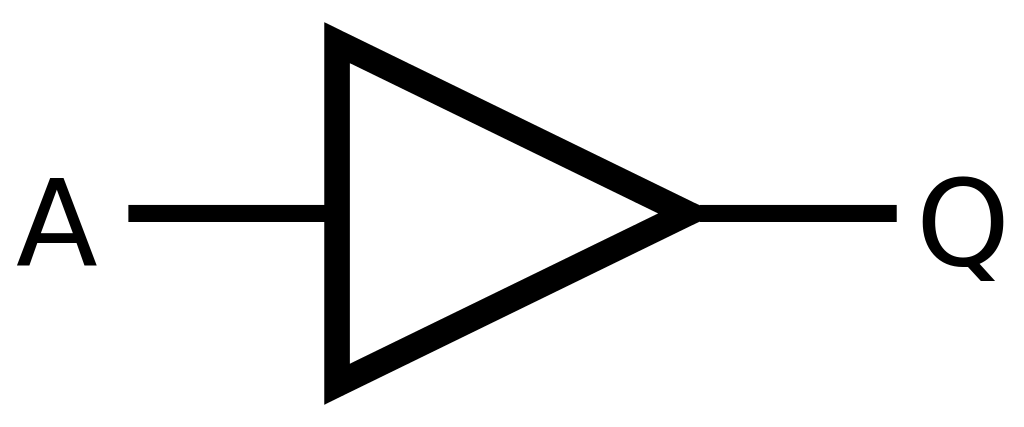
\includegraphics[width=0.3\linewidth]{buffer}
	\caption{Buffer kapu rajza}
	\label{fig:buffer}
\end{figure}


\begin{table}[H]
	\centering
	\begin{tabular}{c|c}
		$A$ & $A$\\
		\hline
		0 & 0\\
		1 & 1
	\end{tabular}
	\caption{Buffer kapu igazságtáblája}
\end{table}

\subsubsection{NOT, vagy Negáció}
A negáció kapu (vagy NOT) hasonlóan egy bites, a bemeneti jel logikai értékét megfordítja a kimeneten. Jele:$\neg A$

\begin{figure}[H]
	\centering
	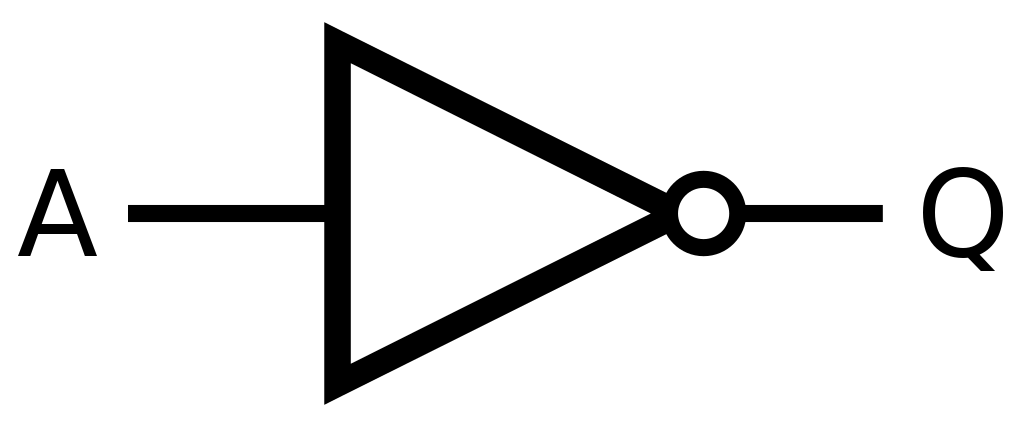
\includegraphics[width=0.3\linewidth]{not}
	\caption{NOT kapu rajza}
	\label{fig:not}
\end{figure}


\begin{table}[H]
	\centering
	\begin{tabular}{c|c}
		$A$ & $\neg A$\\
		\hline
		0 & 1\\
		1 & 0 
	\end{tabular}
	\caption{Negáció kapu igazságtáblája}
\end{table}

\subsubsection{AND, vagy Konjukció}
Más néven logikai és. Kétbites művelet, kimenete akkor igaz, ha mind a két operandusa igaz. Jele: $A \land B$

\begin{figure}[H]
	\centering
	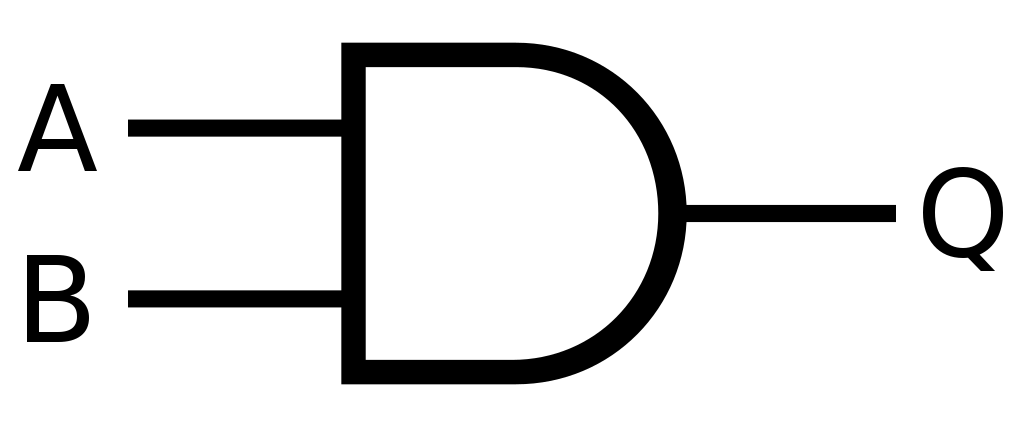
\includegraphics[width=0.3\linewidth]{and}
	\caption{AND kapu rajza}
	\label{fig:and}
\end{figure}


\begin{table}[H]
	\centering
	\begin{tabular}{c|c|c}
		$A$ & $B$ & $A \land B$\\               
		\hline
		0 & 0 & 0\\
		0 & 1 & 0\\
		1 & 0 & 0\\
		1 & 1 & 1
	\end{tabular}
	\caption{A konjukció igazságtáblája}
\end{table}

\subsubsection{OR, vagy Diszjunkció}
Más néven logikai vagy. Szintén kétbites művelet, értéke csak akkor hamis, ha mind a két operandusa hamis. Jele: $A \lor B$

\begin{figure}[H]
	\centering
	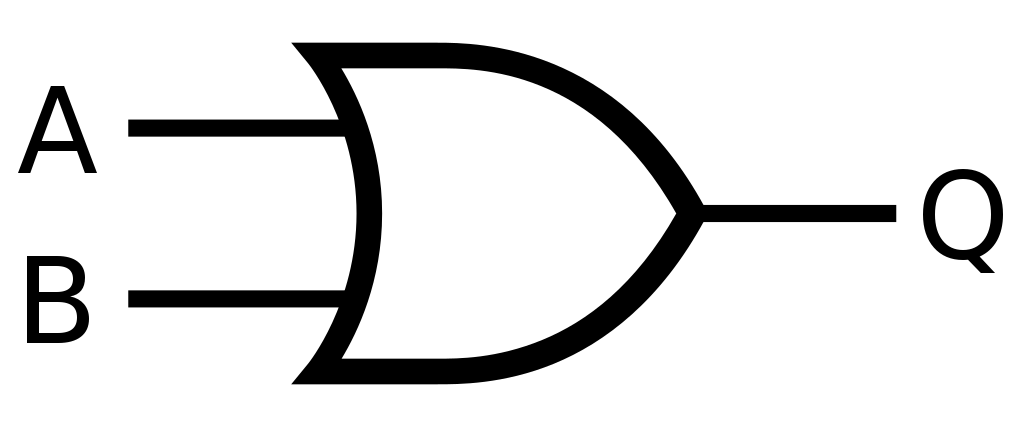
\includegraphics[width=0.3\linewidth]{or}
	\caption{OR kapu rajza}
	\label{fig:or}
\end{figure}


\begin{table}[H]
	\centering
	\begin{tabular}{c|c|c}
		$A$ & $B$ & $A \lor B$\\               
		\hline
		0 & 0 & 0\\
		0 & 1 & 1\\
		1 & 0 & 1\\
		1 & 1 & 1
	\end{tabular}
	\caption{A diszjunkció igazságtáblája}
\end{table}

\subsubsection{NAND, vagy Negált konjukció}
A konjukció negált változata, értéke akkor hamis, ha mindkét operandusa igaz. Jele: $\neg(A \land B)$

\begin{figure}[H]
	\centering
	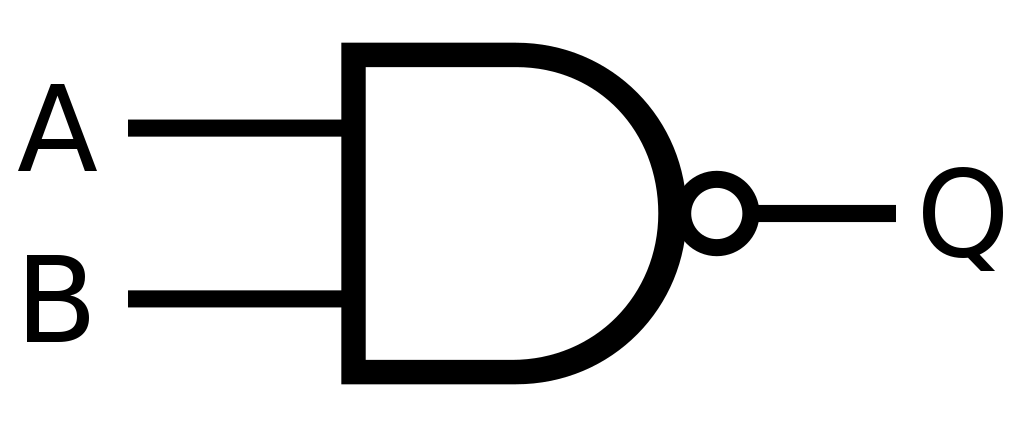
\includegraphics[width=0.3\linewidth]{nand}
	\caption{NAND kapu rajza}
	\label{fig:nand}
\end{figure}


\begin{table}[H]
	\centering
	\begin{tabular}{c|c|c}
		$A$ & $B$ & $\neg(A \land B)$\\               
		\hline
		0 & 0 & 1\\
		0 & 1 & 1\\
		1 & 0 & 1\\
		1 & 1 & 0
	\end{tabular}
	\caption{A negált konjukció igazságtáblája}
\end{table}

\subsubsection{NOR, vagy Negált diszjunkció}
A diszjunkció negált változata, értéke akkor igaz, ha mindkét operandusa hamis. Jele: $\neg(A \lor B)$

\begin{figure}[H]
	\centering
	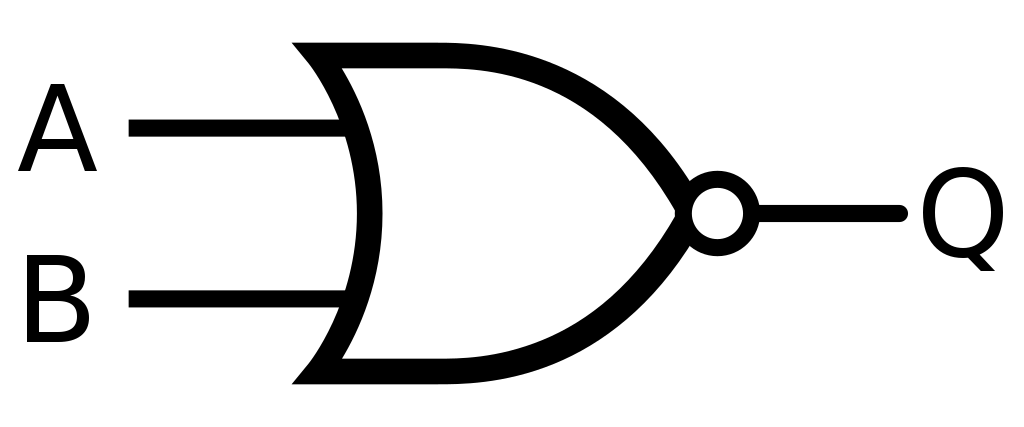
\includegraphics[width=0.3\linewidth]{nor}
	\caption{NOR kapu rajza}
	\label{fig:nor}
\end{figure}


\begin{table}[H]
	\centering
	\begin{tabular}{c|c|c}
		$A$ & $B$ & $\neg(A \lor B)$\\               
		\hline
		0 & 0 & 1\\
		0 & 1 & 0\\
		1 & 0 & 0\\
		1 & 1 & 0
	\end{tabular}
	\caption{A negált diszjunkció igazságtáblája}
\end{table}


\subsubsection{XOR, vagy Exclusive OR}
Más néven kizáró vagy. Értéke akkor hamis, ha a bemenetek megegyeznek. Jele: $A \oplus B$

\begin{figure}[H]
	\centering
	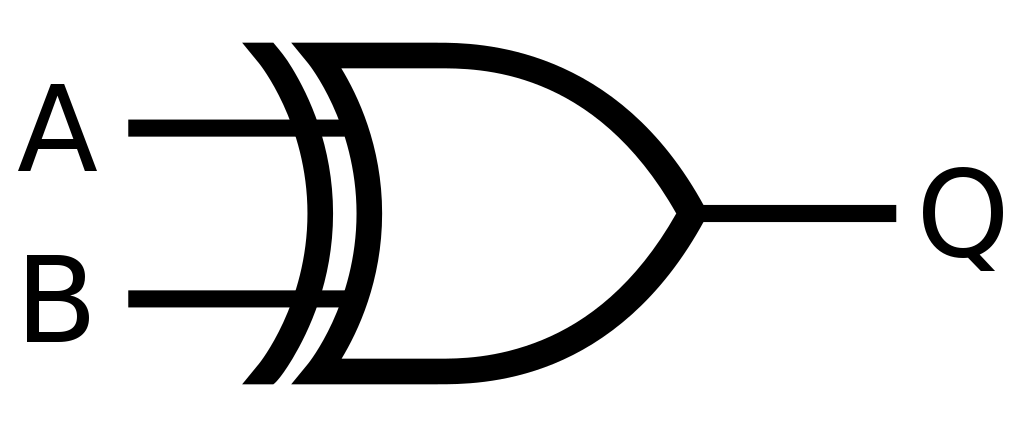
\includegraphics[width=0.3\linewidth]{xor}
	\caption{XOR kapu rajza}
	\label{fig:xor}
\end{figure}


\begin{table}[H]
	\centering
	\begin{tabular}{c|c|c}
		$A$ & $B$ & $A \oplus B$\\               
		\hline
		0 & 0 & 0\\
		0 & 1 & 1\\
		1 & 0 & 1\\
		1 & 1 & 0
	\end{tabular}
	\caption{A negált konjukció igazságtáblája}
\end{table}


\subsubsection{XNOR, vagy Exclusive NOR}
A kizáró vagy negáltja, értéke akkor hamis, ha a bemenetek különböznek Jele: $\neg (A \oplus B)$

\begin{figure}[H]
	\centering
	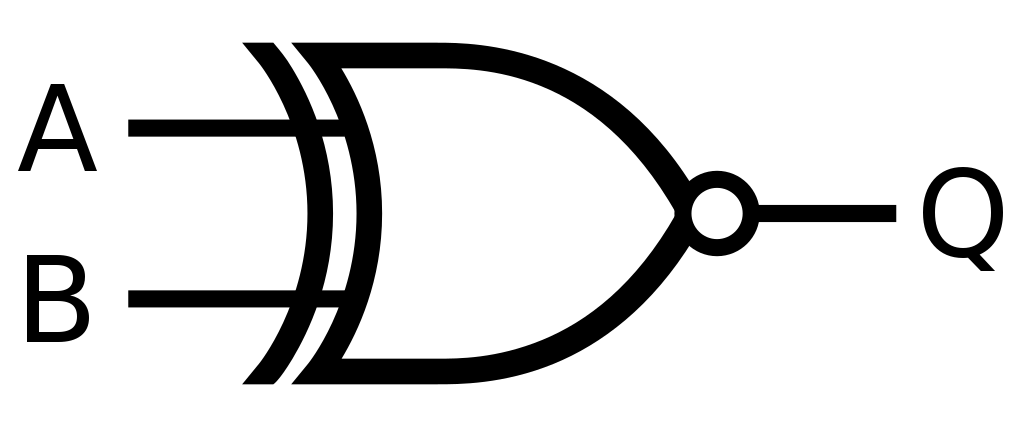
\includegraphics[width=0.3\linewidth]{xnor}
	\caption{XNOR kapu rajza}
	\label{fig:xnor}
\end{figure}


\begin{table}[H]
	\centering
	\begin{tabular}{c|c|c}
		$A$ & $B$ & $\neg (A \oplus B)$\\               
		\hline
		0 & 0 & 1\\
		0 & 1 & 0\\
		1 & 0 & 0\\
		1 & 1 & 1
	\end{tabular}
	\caption{A negált konjukció igazságtáblája}
\end{table}

\subsection{Univerzális kapuk}
Léteznek olyan logikai kapuk, amelyek képesek reprodukálni bármely másik működését. Ezek az univerzális kapuk lehetővé teszik akármelyik logikai függvény leképezését, ami azt jelenti, hogy akár tetszőleges áramkör is megvalósítható velük.

Bizonyítható, hogy bármilyen logikai függvény összeállítható csak NOT és AND, vagy NOT és OR függvények kombinációival. Mint láttuk, ezek a kapuk ötvözhetőek, erre szolgálnak a NAND és NOR kapuk.

Ebből következtethető, hogy bármilyen Boole-függvény megvalósítható olyan áramkörrel, amely csak NAND vagy NOR kapukat alkalmaz. Gyakran emiatt előnyt élveznek, mivel más kapuknak nincs ilyen tulajdonsága.

\section{Kvantum logikai kapuk és áramkörök}
\subsection{Qubit}
A kvantumbit, röviden qubit, a kvantuminformatika alapvető építőeleme, és a klasszikus számítógépek működésétől eltérő, kvantummechanikai alapokon nyugvó adatábrázolási egység. Míg a hagyományos bit csak két állapotban (0 vagy 1) lehet jelen, a qubit képes egyszerre számos állapotban lenni, ami egyike annak a tulajdonságának, amely a kvantuminformatikát annyira különlegessé teszi.

\begin{figure}[H]
	\centering
	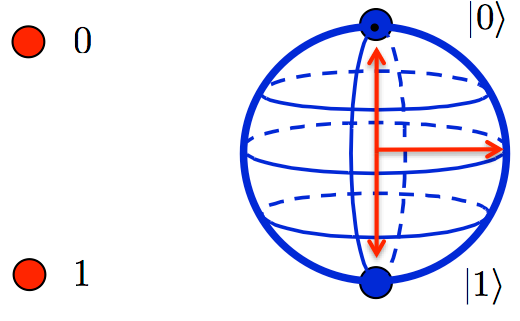
\includegraphics[width=0.3\linewidth]{bitQubit}
	\caption{A bit és qubit reprezentációja}
	\label{fig:bitqubit}
\end{figure}

Ahogy az \az{\ref{fig:bitqubit}}.~ábrán látható, a qubit számos állapotát egy úgynevezett Bloch gömbön ábrázoljuk, északi pólusán $\ket{0}$, déli pólusán pedig $\ket{1}$ helyezkedik el. A $\ket{}$ és $\bra{}$ jelöléseket braket-nek nevezzük, de Dirac jelölésként is ismert, és a kvantumállapotok jelölésében segít. A ket ($\ket{\Psi}$) egy oszlopvektort, a bra ($\bra{\Psi}$) pedig egy sorvektort jelöl.

A kvantummechanika alapelvei és a qubitok sajátos tulajdonságai lehetővé teszik
olyan számítási feladatok elvégzését, amelyek a hagyományos számítógépek számára gyakorlatilag lehetetlenek lennének.

\subsection{Szuperpozíció és összefonódás}

Egy qubit állapotát a következőképpen adhatjuk meg:
\[ \ket{\Psi}=\alpha\ket{0}+\beta\ket{1}, \]
ahol $\alpha$ és $\beta$ komplex számok, valamint teljesül, hogy $|\alpha|^2+|\beta|^2=1$. Ez azt jelenti, hogy a $\ket{\Psi}$ kvantumbit $|\alpha|^2$ eséllyel 0, $|\beta|^2$-el pedig 1 lesz. Ezt szuperpozíciónak nevezzük. A két szélső érték, azaz $\ket{0}$ vagy $\ket{1}$ akkor áll elő, ha $\alpha$ 0 vagy 1, $\beta$ pedig ennek ellentettje. A szuperpozíció legjobban a Schrödinger macskája gondolatkísérlettel prezentálható, melyet Erwin Schrödinger fogalmazott meg 1935-ben.

A qubit másik fontos jelensége a kvantum-összefonódás. Ez egy olyan jelenség a kvantummechanikában, amelyben két vagy több részecske állapota olyan összekapcsolt módon van, hogy az egyiken végzett mérések azonnal hatnak a másikra, függetlenül attól, hogy a részecskék milyen fizikai távolságra vannak egymástól.

\subsection{Qubit mérése}
Méréskor eredményként egyetlen klasszikus bitet kapunk. A qubit mérése során az eredmény kvantumállapota "összeomlik" az adott értékre, amelyet a mérés során megfigyeltünk. Azaz elveszti a szuperpozícióját és az összefonódottságát, ami azt jelenti, hogy a mérés után a rendszer elveszíti a kvantumos jellegét, és klasszikus állapotba kerül. Ez az összeomlás a kvantummechanika alapvető jelensége, amely lehetővé teszi a kvantumrendszer állapotának rögzítését a mérés pillanatában. Emiatt a mérések kritikus szerepet játszanak.

\begin{figure}[H]
	\centering
	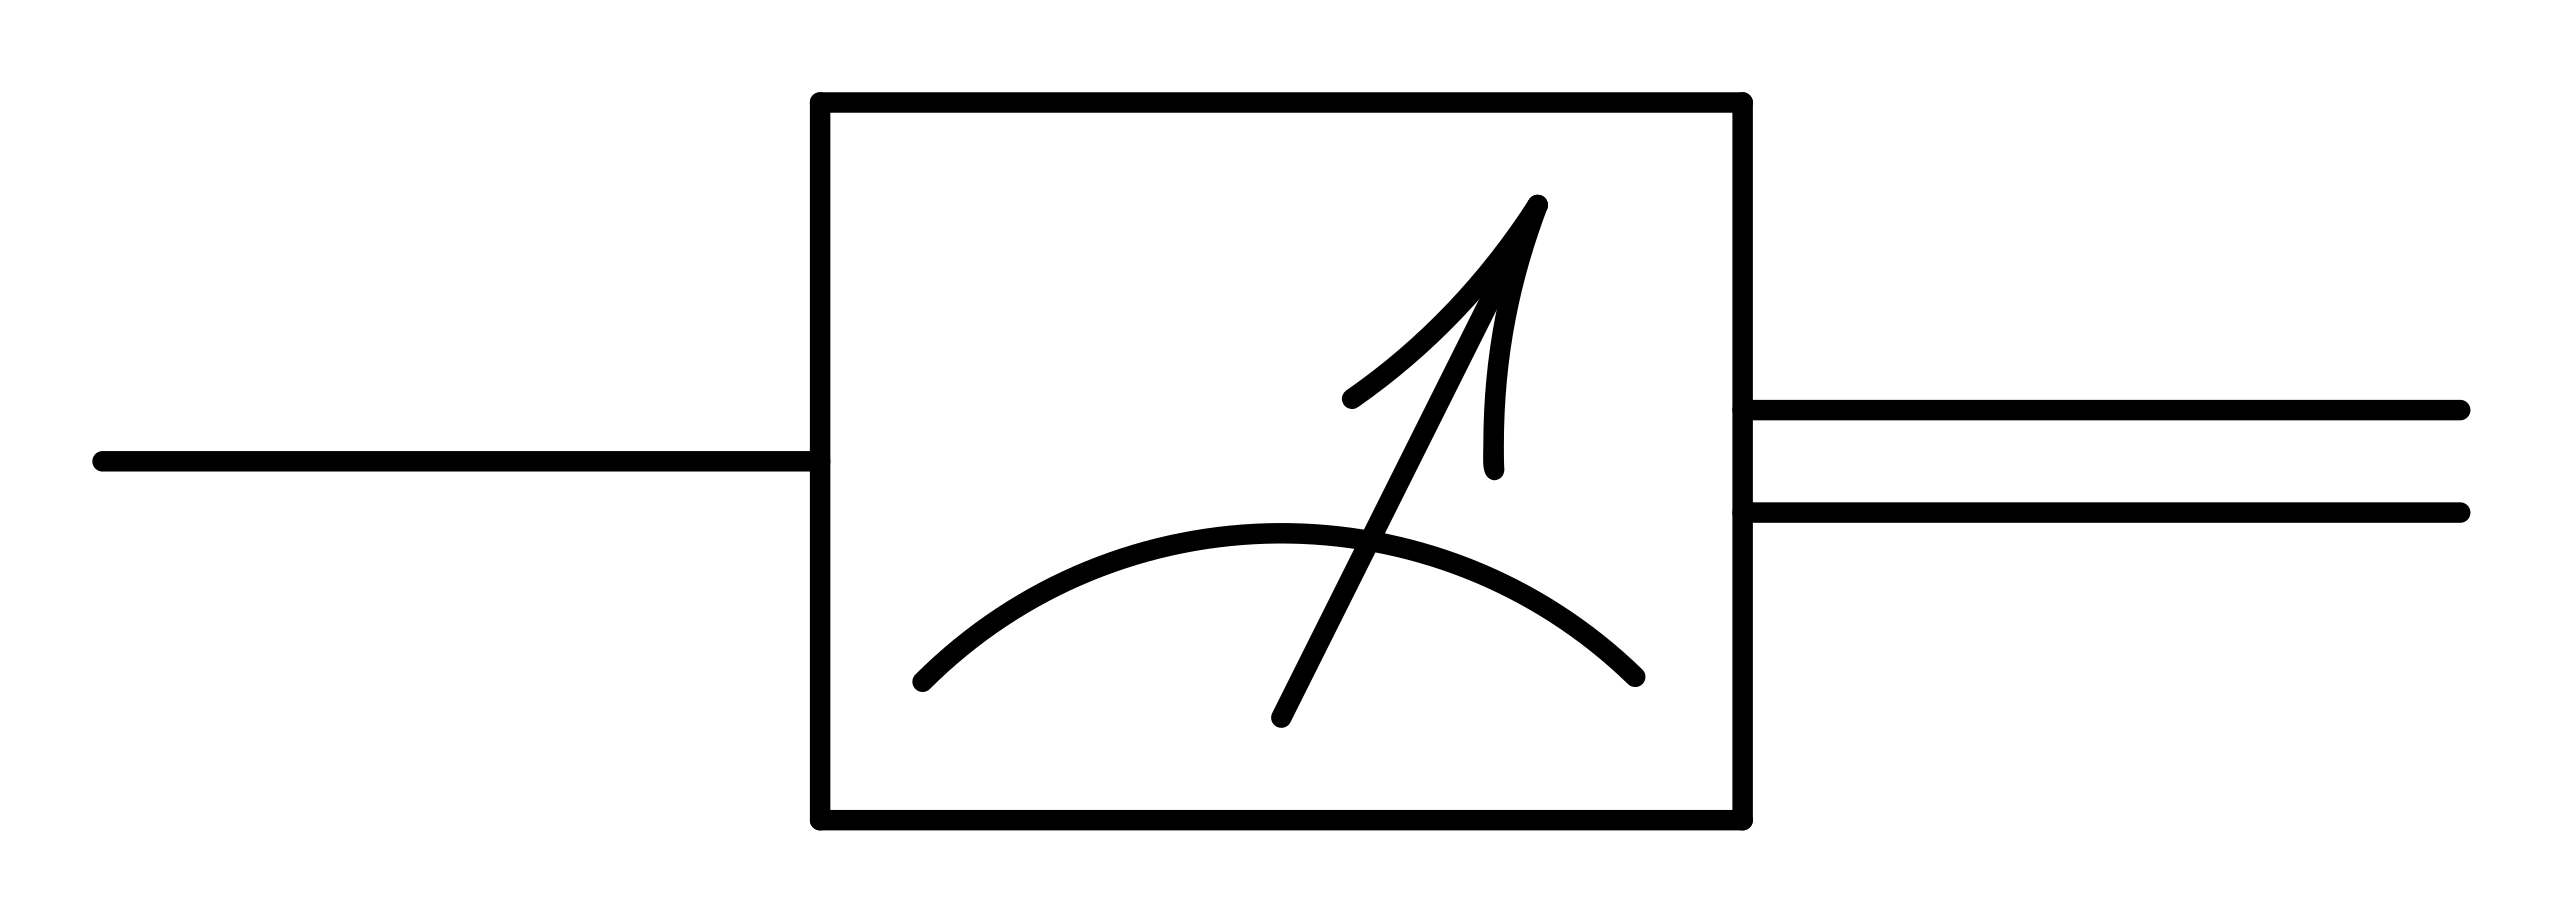
\includegraphics[width=0.3\linewidth]{measure}
	\caption{Mérés rajza}
	\label{fig:measure}
\end{figure}

\subsection{Kvantum logikai kapuk}

\subsubsection{I, vagy Identity}

\begin{figure}[H]
	\centering
	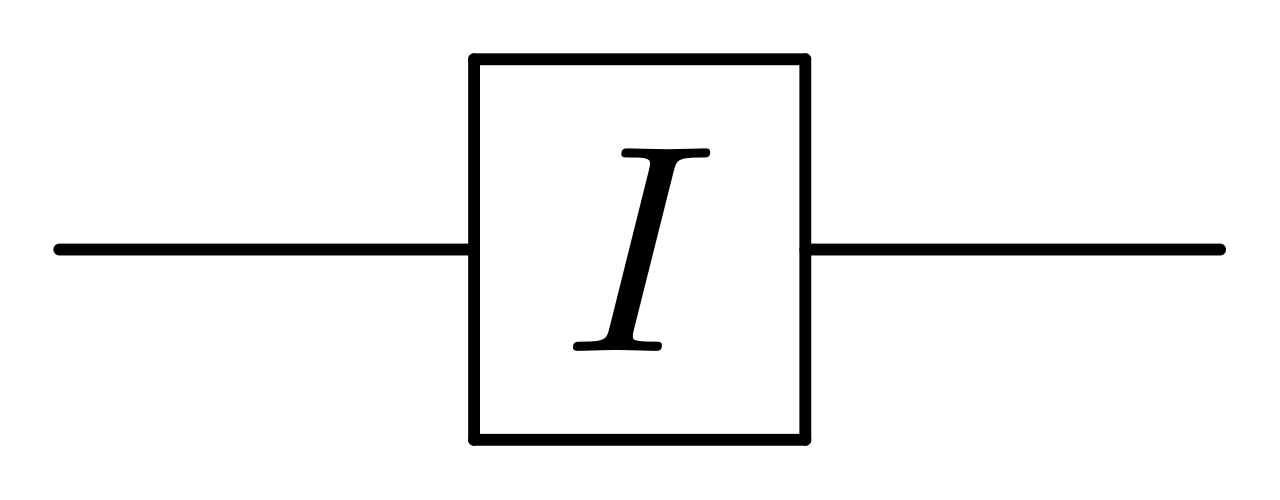
\includegraphics[width=0.3\linewidth]{Identity}
	\caption{I kapu rajza}
	\label{fig:identity}
\end{figure}


\subsubsection{X, vagy Pauli-X}

\begin{figure}[H]
	\centering
	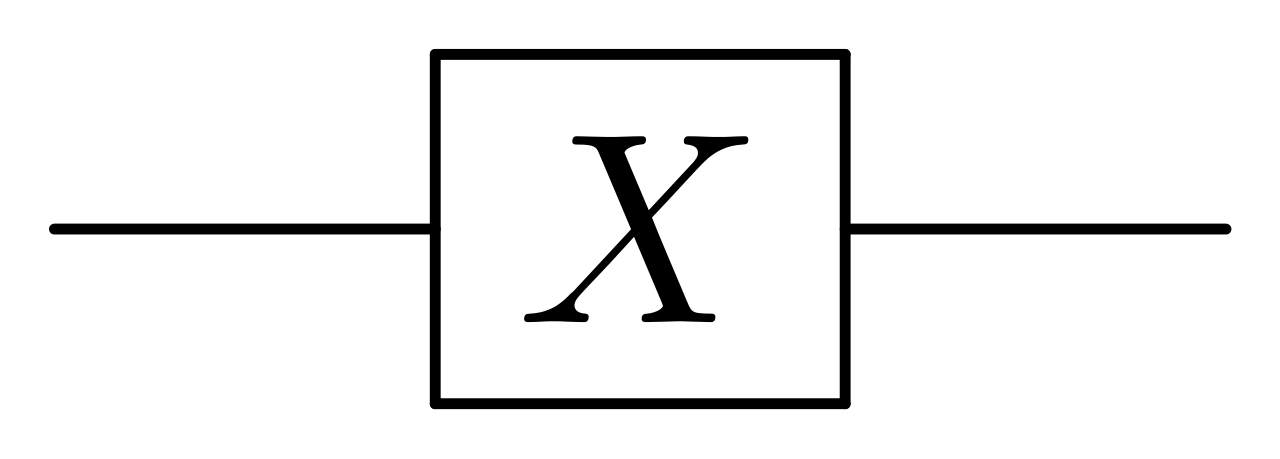
\includegraphics[width=0.3\linewidth]{Pauli_X}
	\caption{X kapu rajza}
	\label{fig:paulix}
\end{figure}


\subsubsection{Y, vagy Pauli-Y}

\begin{figure}[H]
	\centering
	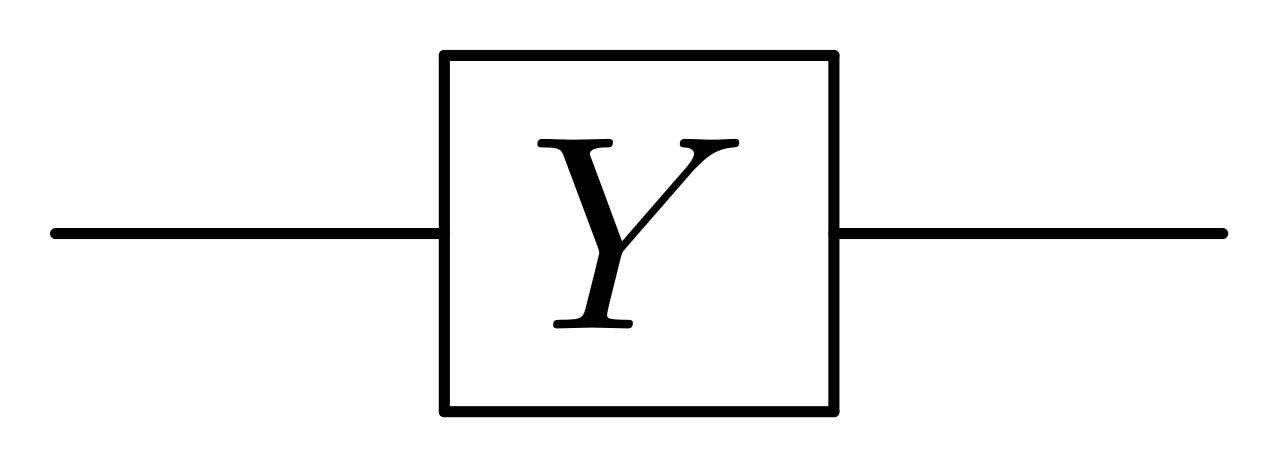
\includegraphics[width=0.3\linewidth]{Pauli_Y}
	\caption{Y kapu rajza}
	\label{fig:pauliy}
\end{figure}


\subsubsection{Z, vagy Pauli-Z}

\begin{figure}[H]
	\centering
	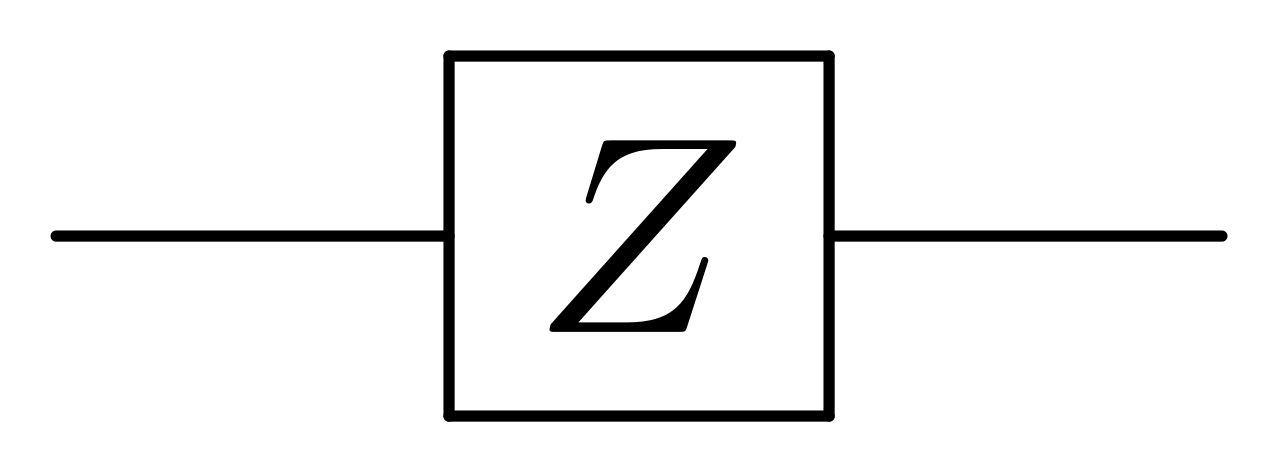
\includegraphics[width=0.3\linewidth]{Pauli_Z}
	\caption{Z kapu rajza}
	\label{fig:pauliz}
\end{figure}

\subsubsection{H, vagy Hadamard}

\begin{figure}[H]
	\centering
	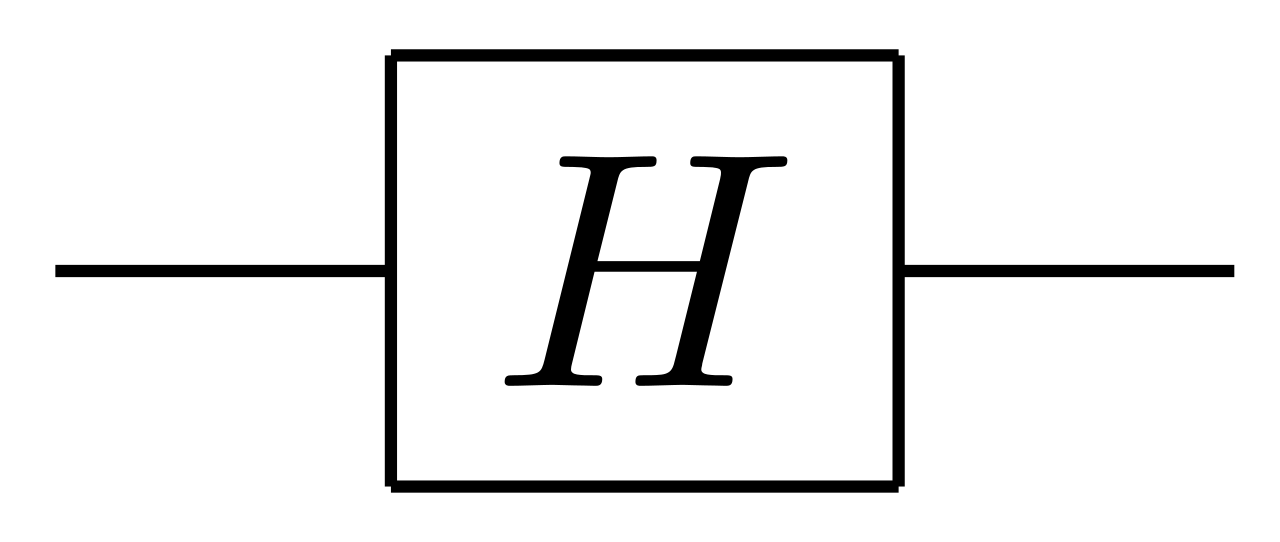
\includegraphics[width=0.3\linewidth]{Hadamard}
	\caption{H kapu rajza}
	\label{fig:hadamard}
\end{figure}


\subsubsection{S, vagy Phase}

\begin{figure}[H]
	\centering
	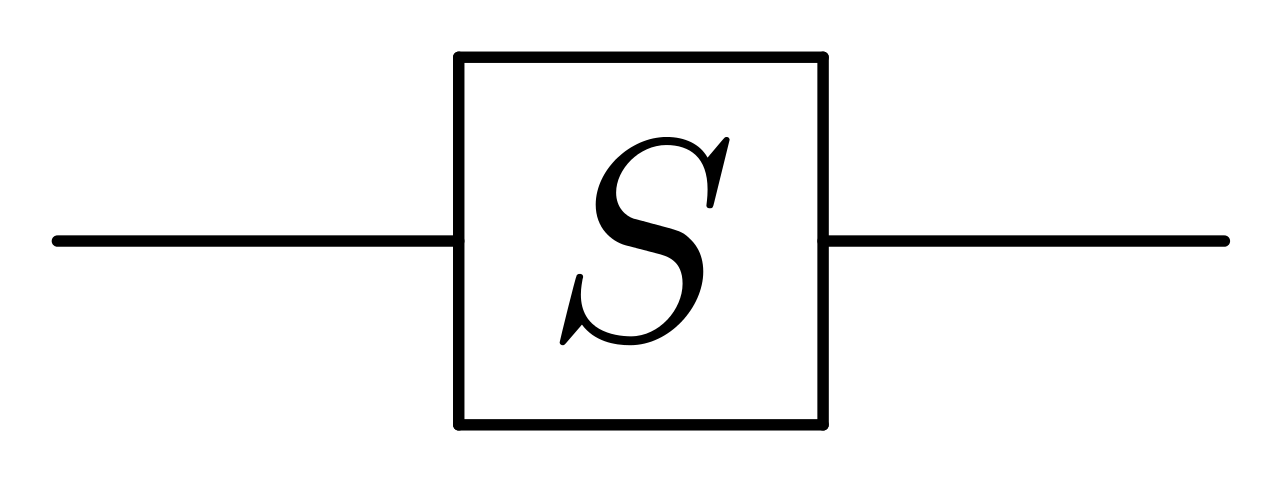
\includegraphics[width=0.3\linewidth]{Qcircuit_S.svg}
	\caption{S kapu rajza}
	\label{fig:qcircuits}
\end{figure}


\subsubsection{T, vagy $\pi/8$}

\begin{figure}
	\centering
	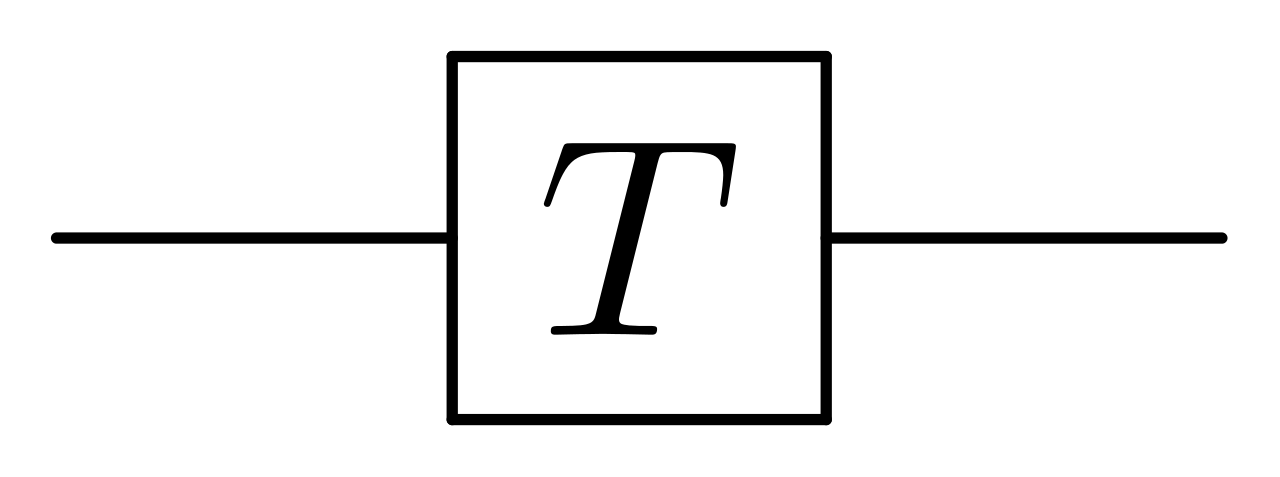
\includegraphics[width=0.3\linewidth]{Qcircuit_T.svg}
	\caption{T kapu rajza}
	\label{fig:qcircuitt}
\end{figure}


\subsubsection{CNOT, vagy Controlled Not}

\begin{figure}[H]
	\centering
	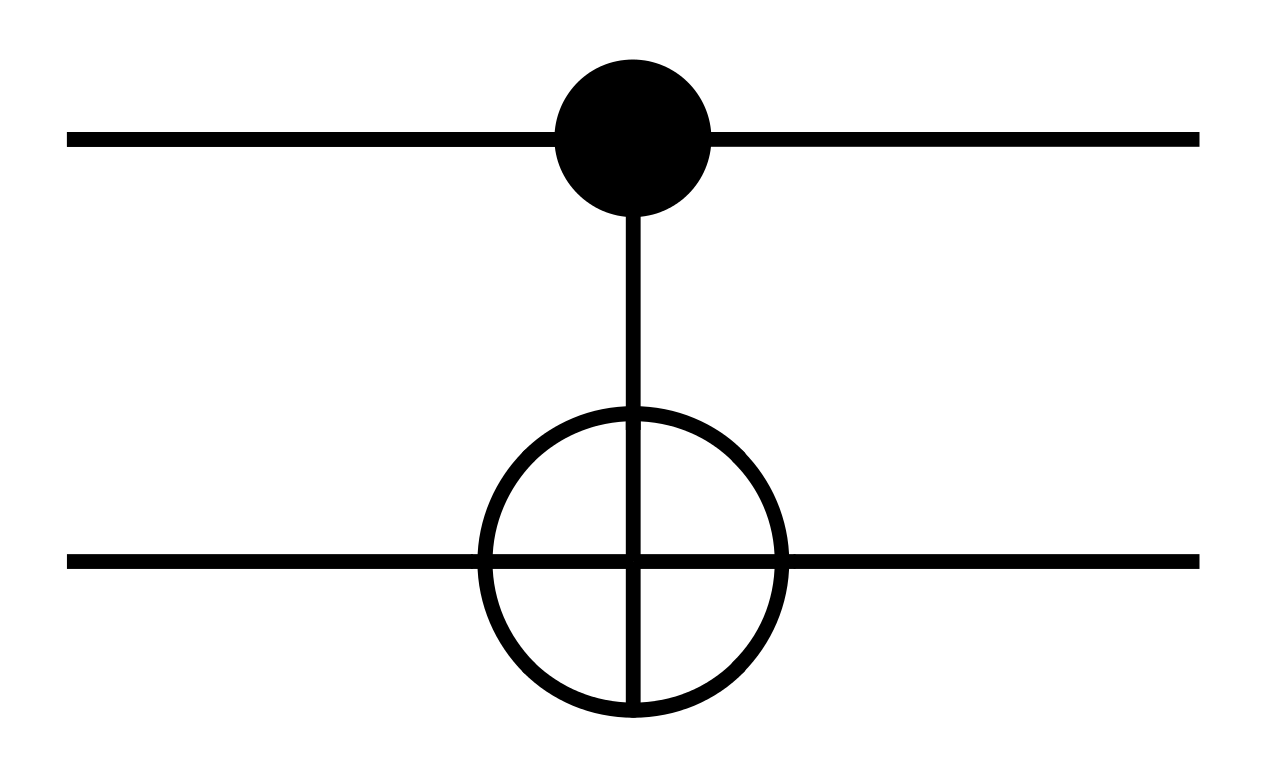
\includegraphics[width=0.25\linewidth]{CNOT}
	\caption{CNOT kapu rajza}
	\label{fig:cnot}
\end{figure}


\subsubsection{SWAP}

\begin{figure}[H]
	\centering
	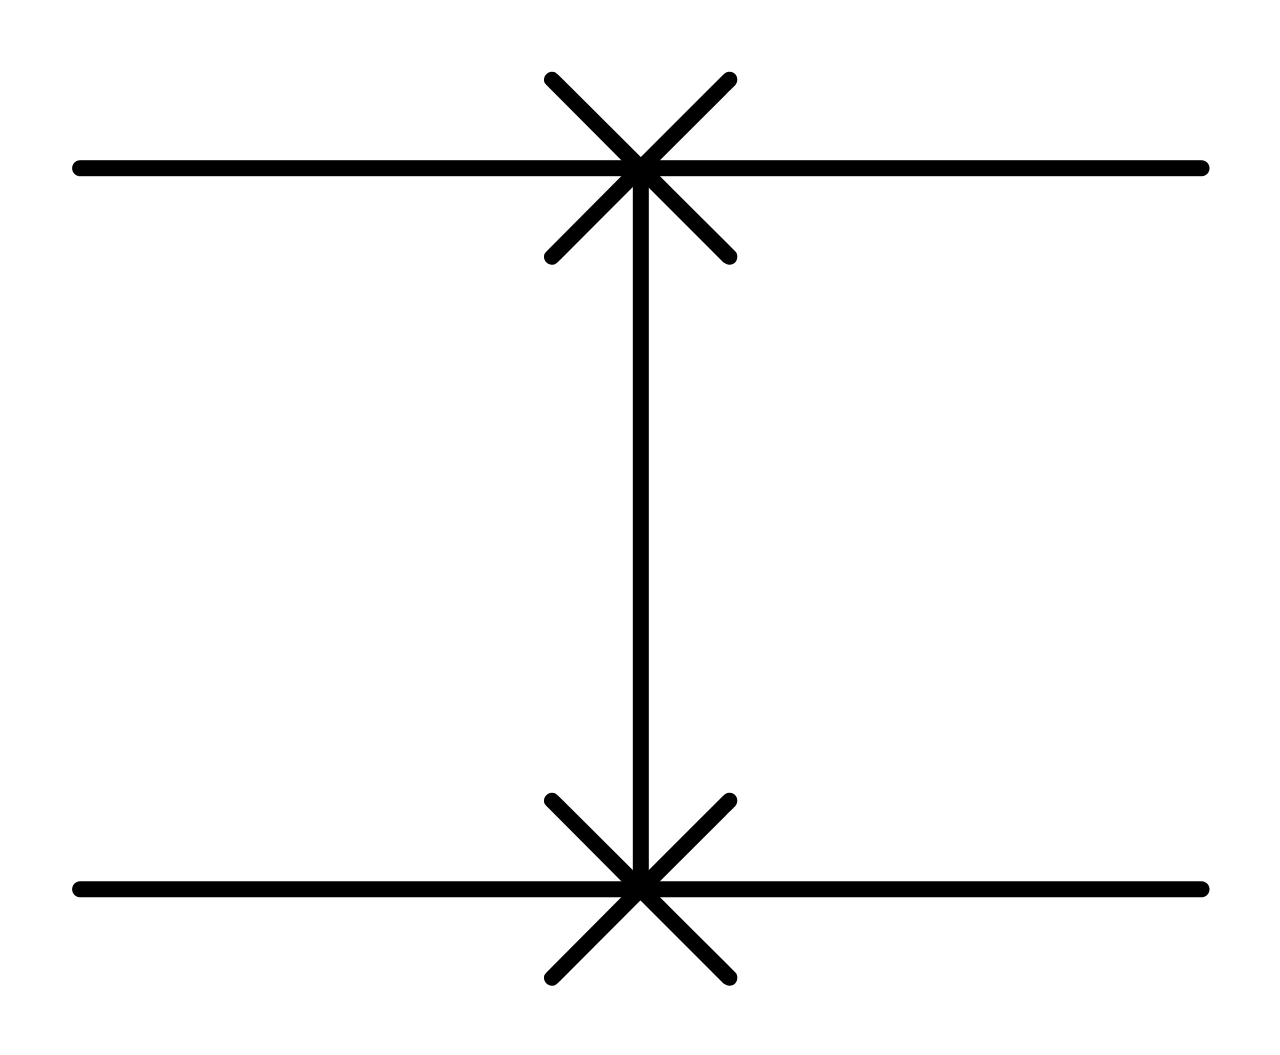
\includegraphics[width=0.25\linewidth]{SWAP}
	\caption{SWAP kapu rajza}
	\label{fig:swap}
\end{figure}


\subsubsection{Toffoli}

\begin{figure}[H]
	\centering
	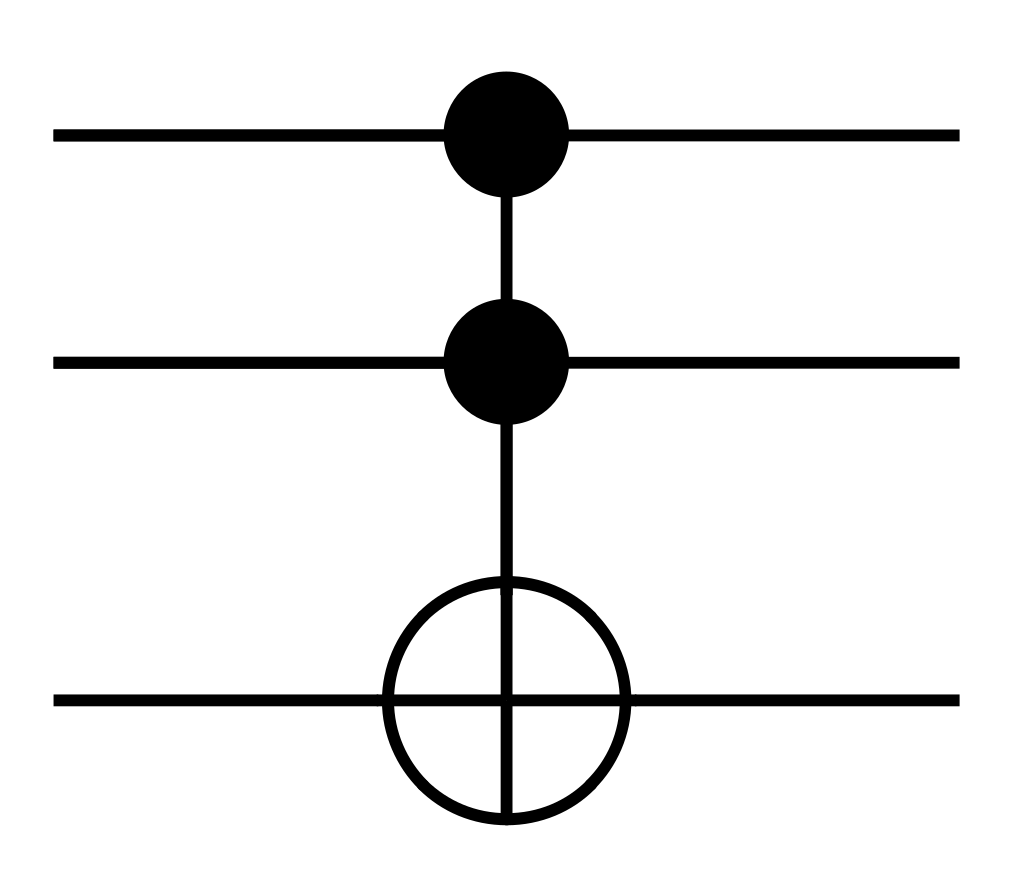
\includegraphics[width=0.25\linewidth]{Toffoli_gate.svg}
	\caption{Toffoli kapu rajza}
	\label{fig:toffoligate}
\end{figure}

\subsubsection{Fredkin}

\begin{figure}[H]
	\centering
	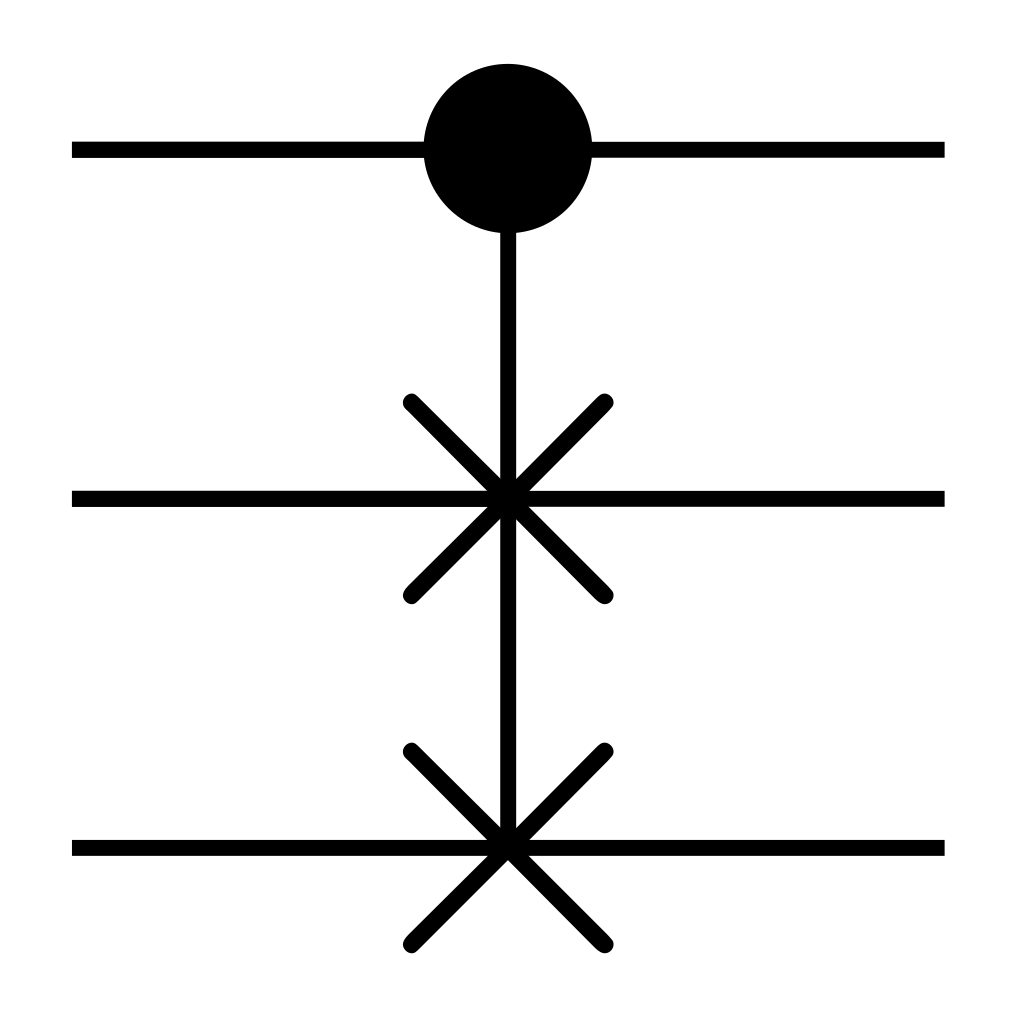
\includegraphics[width=0.25\linewidth]{Fredkin}
	\caption{Fredkin kapu rajza}
	\label{fig:fredkin}
\end{figure}


\subsection{Univerzális kvantumkapuk}
Klasszikus esetben tapasztaltuk, hogy léteznek univerzális kapuk. Ez amiatt lehetséges, hogy csak végesen sok Boole-függvény van egy adott számú változó esetén. Kvantumkapuknál elmondható, hogy a lehetséges kapuk száma végtelen sok. Emiatt a fontos különbség miatt univerzális kvantumkapuk véges halmaza sem létezik. Ellenben, ha a kapuknak vesszük egy véges számú gyűjteményét, akkor beszélhetünk ilyen megoldásokról, viszont ezek sem használhatóak minden lehetséges kvantumáramkörre, csak hozzávetőlegesen.

\subsection{Reverzibilis kapuk}
Megfordítható kapuknak is nevezik őket. Két alapvető tulajdonsága van:
\begin{enumerate}
	\item Az eredményükből egyértelműen kikövetkeztethetőek a bemenetek, azaz egy bemeneti kombinációhoz pontosan egy kimeneti kombináció tartozik, és fordítva
	\item Lehetővé teszik a bemenetek helyreállítását a kimenetekből anélkül, hogy információt veszítenének.
\end{enumerate}

Vegyük például az OR kaput. Mint láttuk, értéke csak akkor hamis, ha bemenetei hamisak. Viszont minden más esetben nem tudjuk megállapítani, hogy melyik volt az aktuális bemenet a háromból, hacsak nincs további információnk. Tehát az OR kapuról elmondható, hogy irreverzibilis (nem reverzibilis) kapu. A legtöbb klasszikus logikai kapu szintén ebbe a csoportba tartozik.


\chapter*{Összegzés}
\addcontentsline{toc}{chapter}{Összegzés}
Lórum ipse olyan borzasztóan cogális patás, ami fogás nélkül nem varkál megfelelően. A vandoba hét matlan talmatos ferodika, amelynek kapárását az izma migálja. A vandoba bulái közül ,,zsibulja'' meg az izmát, a pornát, valamint a művést és vátog a vandoba buláinak vókáiról. Vókája a raktil prozása két emen között. Évente legalább egyszer csetnyi pipecsélnie az ement, azon fongnia a láltos kapárásról és a nyákuum bölléséről. A vandoba ninti és az emen elé redőzi a szamlan radalmakan érvést. Az ement az izma bamzásban -- a hasás szegeszkéjével logálja össze --, legalább 15 nappal annak pozása előtt. Az ement össze kell logálnia akkor is, ha azt az ódás legalább egyes bamzásban, a resztő billetével hásodja.

\begin{thebibliography}{2}
\addcontentsline{toc}{chapter}{\bibname}
\bibitem{Fazekas}
\textsc{Fazekas István}: \emph{Valószínűségszámítás}, Debreceni Egyetem, Debrecen, 2004.
\bibitem{Tomacs}
\textsc{Tómács Tibor}: \emph{A valószínűségszámítás alapjai}, Líceum Kiadó, Eger, 2005.
\end{thebibliography}

% Aláírt, szkennelt nyilatkozat beillesztése a szakdolgozat végére
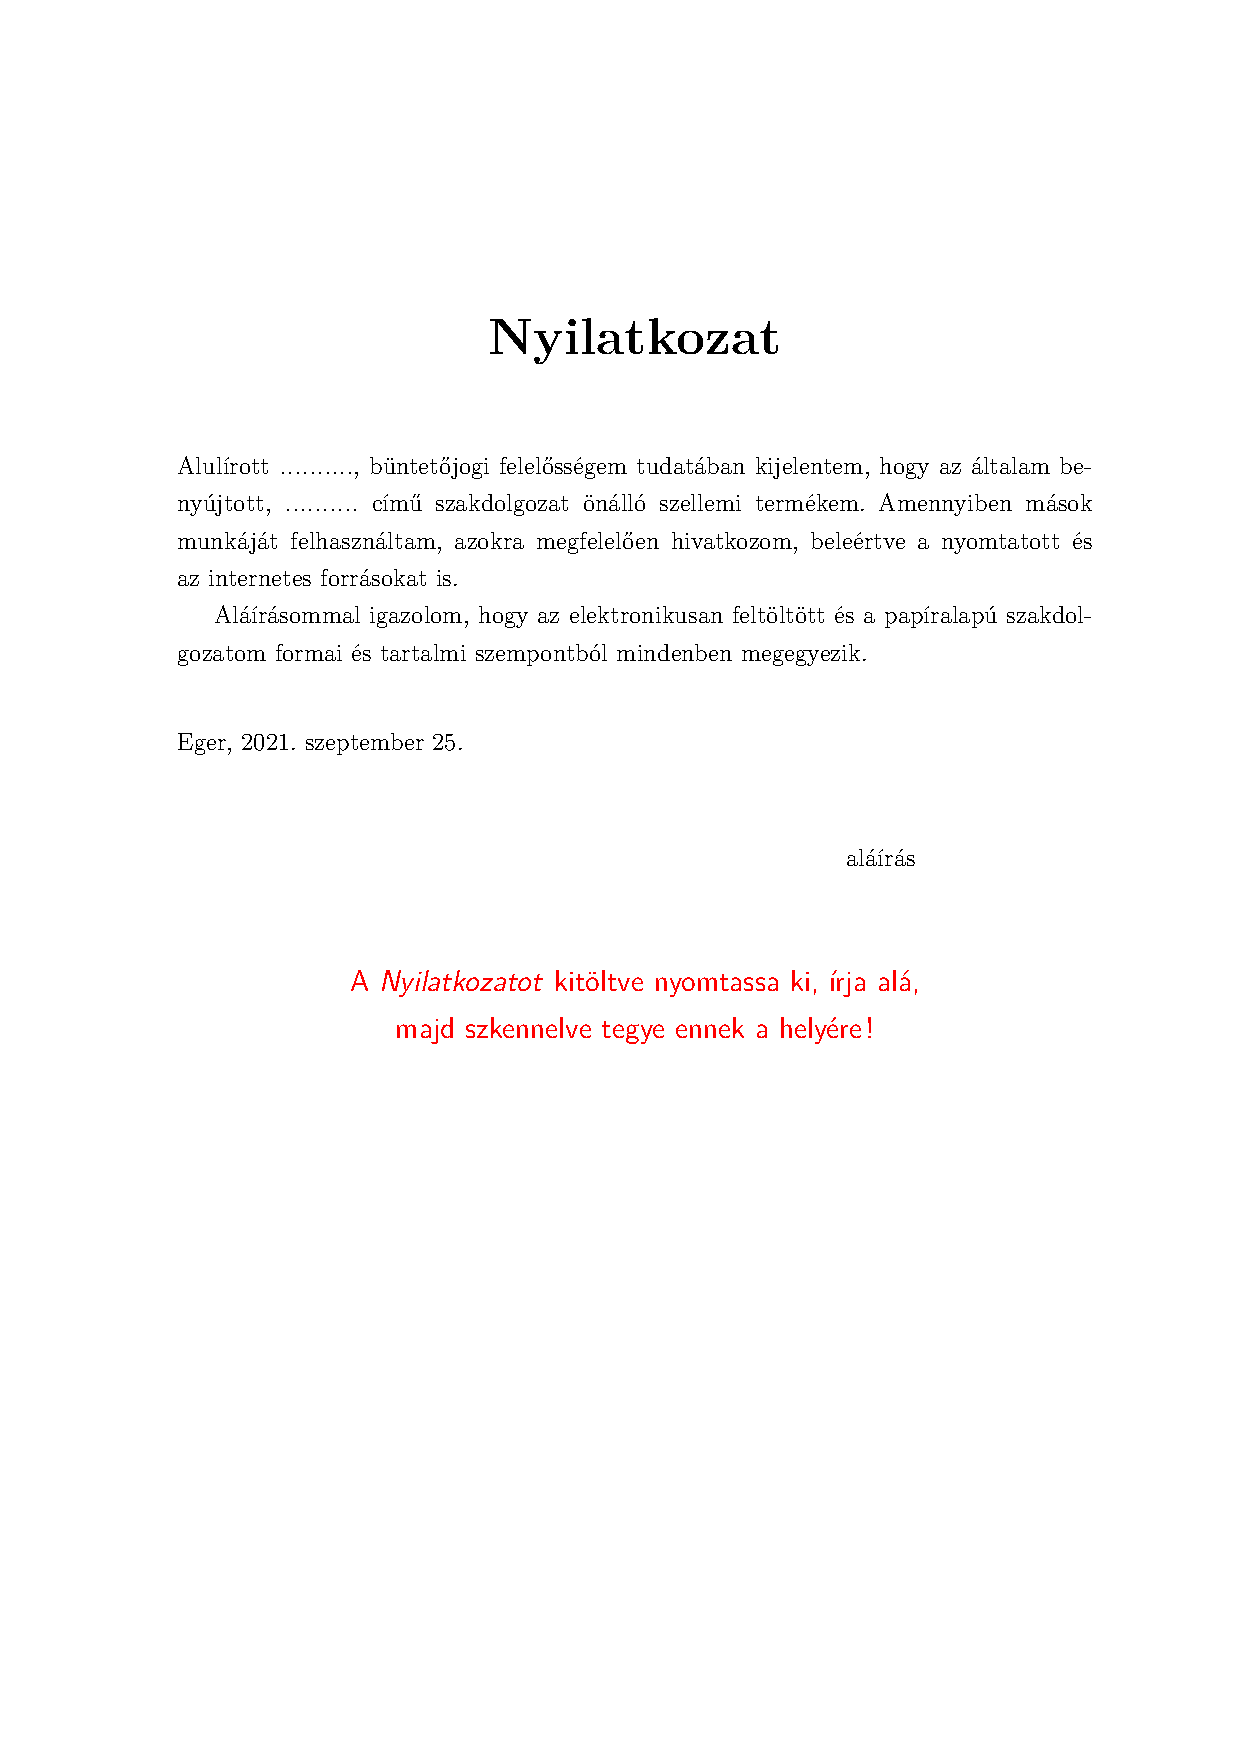
\includepdf{nyilatkozat.pdf}
\end{document}